\documentclass{article}
\usepackage[utf8]{inputenc}
\usepackage{amsmath,amsthm,amsfonts,amssymb,amscd}
\usepackage[a4paper,hmargin=0.8in,bottom=1.3in]{geometry}
\usepackage{lastpage,enumerate,fancyhdr,mathrsfs,graphicx,listings,hyperref,enumitem,listings}
\usepackage[dvipsnames]{xcolor}
\newcommand{\citem}[1]{\item \texttt{#1}}
\newcommand{\dsr}[5]{
\hline 
\texttt{#1} & #2 & #3 & #4 & #5\\
}
\newcommand{\specialcell}[2][c]{%
  \begin{tabular}[#1]{@{}c@{}}#2\end{tabular}}
\author{Hardik Rajpal}
\title{Notes from nearly draining pursuits\\of mastery in Leetcode problems}
\hbadness 100001
\begin{document}
\definecolor{codegreen}{rgb}{0,0.6,0}
\definecolor{codegray}{rgb}{0.5,0.5,0.5}
\definecolor{codepurple}{rgb}{0.58,0,0.82}
\definecolor{backcolour}{rgb}{0.95,0.95,0.92}

\lstdefinestyle{mystyle}{
    backgroundcolor=\color{backcolour},   
    commentstyle=\color{codegreen},
    keywordstyle=\color{magenta},
    numberstyle=\tiny\color{codegray},
    stringstyle=\color{codepurple},
    basicstyle=\ttfamily\footnotesize,
    breakatwhitespace=false,         
    breaklines=true,                 
    captionpos=b,                    
    keepspaces=true,                 
    numbers=left,                    
    numbersep=5pt,                  
    showspaces=false,                
    showstringspaces=false,
    showtabs=false,                  
    tabsize=2
}
\setlist[enumerate,1]{label=\textbf{\arabic*.}}
\lstset{style=mystyle,language=C++}
\maketitle
\tableofcontents
\pagebreak
\section{STL}
\subsection{Sets and Maps}
These (\texttt{set} and \texttt{map}) are ordered data structures; helpful when
it is efficient to retain the ordering of a collection of elements during execution.
Their unordered counterparts (\texttt{unordered\_set} and \texttt{unorderd\_map})
prioritize access time and maintain no order of their elements.
\subsubsection*{Declaration syntaxes}
\begin{lstlisting}[caption={Sets and Maps},language=C++]
struct U{
    bool operator()(T t1, T t2)const{
        //logic comparing t1<t2.
    }
};
set<T,struct U> myset; multiset<T,struct U> mymulset;
map<T,V,struct U> mymap; multimap<T,struct U> mymulmap;
\end{lstlisting}
The ordering parameter \texttt{U} is crucial in cases where order between T is not inferable.
\begin{lstlisting}[caption={Unordered sets and maps},language=C++]
struct T{
    ...
    bool operator==(T t2)const{
        //return logic for t2==this.
    }
};
struct hashT{
    size_t operator()(T t)const{
        //std::hash<string or int or double>()(string or int or double)
        //return logic for hashing t. Use ^ << >> ~ | &
        //Note: Easy hash for collection of numbers=> sort, join with ","
    }
};
unordered_set<T,struct hashT> uset;
unordered_map<T,V,struct hashT> umap;
\end{lstlisting}
In the interest of speed and space, and unreadability of code, it might be
preferable to replace sets that only serve to mark and check membership
by flags and bit operations.\\
\begin{center}
    \fbox{\texttt{insert(index)}$\equiv$\texttt{flag|(1<<index)} and \texttt{count(index)}$\equiv$\texttt{flag\&(1<<index)}}
\end{center}
\textbf{Note:} The great thing about sets and maps is the uniqueness of their values.
So, to find the maximum element less than an element, we simply \texttt{find()} the element
in the set and decrement the iterator.
\subsubsection{Erase}
\texttt{erase} can take the value to be erased or the iterator to it. With multisets
and multimaps, using the iterator ensures that the duplicates are not erased,
whereas using the value erases all duplicates. Note that the iterator can't be a
\texttt{reverse\_iterator}; we can't use \texttt{rbegin()} and must use
\texttt{end()} after decrementing it. 
\subsection{Priority Queue}
These structures lazily maintain order between their elements; only 
one extreme of the elements in the data structure is accessible at 
any time. The implementation involves a heap. the usage is as below:
\begin{lstlisting}[caption={Priority Queue},language=C++]
    struct U{
        bool operator()(T t1, T t2)const{
            //logic comparing t1<t2.
        }
    };
    priority_queue<T,vector<T>,struct U> pq;
\end{lstlisting}
The default U is \texttt{std::less<T>}. \texttt{pq.top()} returns
the largest element, based on the comparator.
\subsubsection{Getting the Kth value}
Some problems can ask for the Kth value (largest/smallest) from an
array of \texttt{val}s. These can be implemented
efficiently with PQs as follows:
\begin{lstlisting}[caption={Kth Largest Element},language=C++]
    priority_queue<int,vector<int>,greater<int>> pq;
    //greater=> pq.top == least value of pq.
    pq.push(val[0]);
    for(int i=1;i<val.size();i++){
        if(pq.size()<k){
            pq.push(val[i]);
        }
        else if(pq.top() < val[i]){
            pq.push(val[i]);
            pq.pop();
        }
    }
    return pq.top();
    //size of pq == k, and we have 
    //collected all high elements=>
    //pq.top == least value must be kth largest
\end{lstlisting}
\begin{lstlisting}[caption={Kth Smallest Element},language=C++]
    priority_queue<int,vector<int>,less<int>> pq;
    //less=> pq.top == max value of pq.
    pq.push(val[0]);
    for(int i=1;i<val.size();i++){
        if(pq.size()<k){
            pq.push(val[i]);
        }
        else if(pq.top() > val[i]){
            pq.push(val[i]);
            pq.pop();
        }
    }
    return pq.top();
    //size of pq == k, and we have 
    //collected all low elements=>
    //pq.top == max value must be kth smallest
\end{lstlisting}
The time complexity of these algorithms is
O((\texttt{val.size()})log(k)); it's linear in
\texttt{val.size()}.
An alternative way to maintain the kth element
in a list of elements, where deletion of specific
elements is necessary (but not permitted by the
priority\_queue data structure), we can use two sets.
\begin{lstlisting}[caption=Kth smallest Element,language=C++]
class Kset{
public:
    size_t k;
    multiset<int> trail;//multiset to permit duplicates.
    multiset<int> others;
    Kset(size_t _k){
        k = _k;
    };
    void insert(int e){
        if(trail.size()<k){
            trail.insert(e);
        }
        else{
            if(e<*trail.rbegin()){
                others.insert(*trail.rbegin());
                auto iter = trail.end();iter--;
                trail.erase(iter);
                trail.insert(e);
            }
            else{
                others.insert(e);
             }
        }
    }
    void erase(int e){
        auto iter = others.find(e);
        if(iter!=others.end()){
            others.erase(iter);
            //erase using iterators to avoid
            //erasing all duplicates
        }
        else{
            iter = trail.find(e);
            if(iter!=trail.end()){
                trail.erase(iter);
                trail.insert(*others.begin());
                others.erase(others.begin());
            }
        }
    }
    int top(){
        //returns kth smallest element.
        return *trail.rbegin();
    }
}
\end{lstlisting}
\subsubsection{Procedural PQ functions}
\begin{itemize}
\item A given vector \texttt{a} can be used as a heap in-place without transferring its contents anywhere using the functions below:
\begin{enumerate}
\item \texttt{make\_heap(first, last[, struct comp])}:moves elements in (first,last) container around to make a heap in O(N) time.
\item \texttt{push\_heap(first, last[, struct comp])}:inserts an element in the max heap \\represented by (first,last).
\item \texttt{pop\_heap}:removes the maximum element in the heap formed by (first,last).
\end{enumerate}
\end{itemize}
\subsection{Deque}
This is the most generic form of a container, combining methods for a stack, a queue and a vector (O(1) index accesses) allowing for:
\begin{enumerate}
\item \texttt{push\_front(val)}
\item \texttt{pop\_front()}
\item \texttt{push\_back(val)}
\item \texttt{pop\_back()}
\item \texttt{front()}
\item \texttt{back()}
\item \texttt{d[i]}
\item \texttt{insert(iter,val)}
\end{enumerate}
\subsection{The Big Fat Table of Data Structures}
\hspace*{-2cm}
\begin{tabular}{ |p{3cm}|c|p{3cm}|p{3cm}|p{3cm}| }
\dsr{STL class}{Insertion}{Deletion}{Lookup}{Remarks}
\dsr{vector<T> s}{
    \specialcell{\texttt{void push\_back(T t)}:O(1)\\
    \texttt{void insert(iter pos, T t)} O(n)}
}{\texttt{pop\_back}: O(1)}{\texttt{var[key]}: O(1)}{\texttt{insert} puts \texttt{t} before \texttt{pos}}
\dsr{set<T> s}
{\specialcell{\texttt{void insert(T t)}:\\O(log(s.size()))}}{\specialcell{\texttt{void erase(T t)}:\\O(log(s.size()))}}{\specialcell{\texttt{iter find(T t)}:\\O(log(s.size()))}}{Implemented as a tree.}
\dsr{map<K,V>}
{\specialcell{
    \texttt{void insert(pair<K,V> p)}:\\
    \texttt{var[k] = v;}
}}
{\specialcell{
    \texttt{void erase(K k)}:\\O(log(s.size()))
}}
{\specialcell{\texttt{iter find(K k)}:\\O(log(s.size()))}}
{...}
\dsr{\specialcell{
    \texttt{priority\_queue}\\
    \texttt{<T,vector<T>,U>}}}
{
\specialcell{
    \texttt{pq.push(T t)}\\
    O(log(\texttt{pq.size()}))
}
}{
    \specialcell{
        \texttt{pq.pop()}\\
        O(log(\texttt{pq.size()}))
    }
}
{\texttt{pq.top()} is O(1)}{...}
\hline
\end{tabular}
\subsection{Comparators}
STL provides its own simple comparators: (\texttt{T} can be replaced by
int, vector, etc.)
\begin{itemize}
    \item \texttt{less<T>} for ascending orders.
    \item \texttt{greater<T>} for descending orders.
\end{itemize} Custom comparators are written like so:
\begin{lstlisting}[caption={Comparators},language=C++]
struct U{
    bool operator()(const T& t1,const T& t2)const{
        //logic comparing t1<t2.
    }
};
\end{lstlisting}
Comparators are used as:
\begin{lstlisting}
set<T,struct ComparatorForT> myset;//note: type passed.
sort(v.begin(),v.end(),ComparatorForT());//note: instance passed.
\end{lstlisting}
\subsubsection{\href{https://stackoverflow.com/a/46128321/14681493}{Better Comparators}}
\subsection*{Static Functions}
\begin{lstlisting}
class Solution{
public:
    static vector<int> fm;
    static bool compare(int i1, int i2){
        return fm[i1] < fm[i2] || i1 < i2;
    }
    void solver(){
        set<int,decltype(Solution::compare)*> myset(Solution::compare);
        //decltype return function type,
        //appending * makes it a pointer.
        //The function is passed as an argument to the constructor.
        //or in a sort function:
        sort(inds.begin(),inds.end(),&(Solution::compare));
    }
};
Solution::vector<int> fm = {};
\end{lstlisting}
\subsection{Iterators}
Without going into the non-trivial hierarchy of iterators, note that:
\begin{itemize}
    \item \texttt{iter++} is supported by all iterators.
    \item \texttt{iter += n} is supported by random-access iterators, available with vectors and deques (and maybe others?).
    \item \texttt{void advance(iter,n)} is supported by all iterators: use this instead.
    \item \texttt{iter next(iter,n)} and \texttt{iter prev(iter,n)} is supported by all iterators.
    \item \texttt{distance(iter\_before,iter\_after)} is the more general version of \texttt{iter\_after - iter\_before}.
\end{itemize}
An iterator pointing at an element is ``corrupted" on removing the element.
Hence, any useful data should be copied over from the iterator before removing the element.
\begin{lstlisting}[caption={Undefined behaviour},language=C++]
    lists.erase(*minit);//minit is corrupted
    lists.insert((*minit)->next);
\end{lstlisting}
\begin{lstlisting}[caption={Working code},language=C++]
    lists.insert((*minit)->next);//first use the data.
    lists.erase(*minit);//then erase.
\end{lstlisting}
\subsection{Built-In Utilities}
Note: \texttt{iter} denotes the iterator return type. \texttt{first} and \texttt{last} denote \texttt{.begin()} and \texttt{.end()} iterators.
\begin{itemize}
    \citem{void sort(first,last[, struct comp])} (O(nlogn))
    \citem{void reverse(first,last)} (O(n))
    \citem{void random\_shuffle(first,last)} (O(n))
    \citem{iter max\_element(first,last[,struct comp])} (O(n))
    \citem{iter min\_element(first,last[,struct comp])} (O(n))
    \citem{int|long long|etc accumulate(first,last,init\_val[, function\_to\_combine(int,T)])} (O(n))
    \citem{iter lower\_bound(first,last,value)}(O(logn))
    \begin{itemize}
        \item Returns \texttt{iter} to the smallest element $\geq$ \texttt{value}.
    \end{itemize}
    \citem{iter upper\_bound(first,last,value)} (O(logn))
    \begin{itemize}
        \item Returns \texttt{iter} to the smallest element $>$ \texttt{value}.
    \end{itemize}
    \citem{bool next\_permutation(first,last[, struct comp])} (O(n))
    \begin{itemize}
        \item Updates \texttt{(first,last)} to its next permutation of in ascending order.
        \item Sort \texttt{(first,last)} first to access all permutations.
        \item Use in a \texttt{do-while} loop to avoid missing first permutation.
        \item Returns true if there exists a permutation greater than the current one.
    \end{itemize}
    \citem{bool prev\_permutation(first, last[, struct comp])} (O(n))
    \citem{void nth\_element(first, iteratorToNthElem,last[, struct comp])} (O(sdt::distance(first,last)))
    \begin{itemize}
        \item Alters the array so that *iteratorToNthElem is the nth smallest element.
        \item Modify the comparator to get nth largest element or other variations.
        \item All elements before iteratorToNthElem are less than the nth smallest element.
        \item All elements after iteratorToNthElem are greater than or equal to it.
    \end{itemize}
    \citem{void insert(v1.end(),v2.begin(),v2.end());} (O(v2.size()))
    \begin{itemize}
        \item Appends whole of v2 to end of v1.
    \end{itemize}
\end{itemize}
\section{Graph Algorithms}
\subsection{BFS|DFS}
I prefer writing both of these iteratively. In the immortal
intonation of Ashish Mishra,\\
\textbf{BFS} - \textbf{Queue}\\
\textbf{DFS} - \textbf{Stack}\\
Here's a sample of both algorithms.\\
\noindent\begin{minipage}{.45\textwidth}
    \begin{lstlisting}[caption=BFS,language=C++]
T s;
unordered_map<T,vector<T>> edges;
queue<T> q;
unordered_map<T,bool> visited;
unordered_map<T,T> prev;
int steps = 0;
q.push(s);
visited[s] = true;
while(!q.empty()){
    int sz = q.size();
    while(sz--){
        T u = q.front();
        q.pop();
        for(nb:edges[u]){
            if(!visited[nb]){
               visited[nb] = true;
               prev[nb] = u;
               q.push(nb);
            }
        }
    }
    steps++;
}
        \end{lstlisting}
\end{minipage}\hfill
\begin{minipage}{.45\textwidth}
    \begin{lstlisting}[caption=DFS,language=C++]
    T s;
    unordered_map<T,vector<T>> edges;
    stack<T> s;
    unordered_map<T,bool> visited;
    unordered_map<T,T> prev;
    s.push(s);
    visited[s] = true;
    while(!s.empty()){
        T u = s.top();
        s.pop();
        for(nb:edges[u]){
            if(!visited[nb]){
                visited[nb] = true;
                prev[nb] = u;
                q.push(nb);
            }
        }
    }
    \end{lstlisting}
\end{minipage}\\
The nodes should be reduced from the abstract type T, to
int whenever possible; thereby reducing the
\texttt{unordered\_map}s to \texttt{vector}s which can
sometimes get you under the time limit.
\href{https://stackoverflow.com/questions/55451825/why-is-vector-faster-than-unordered-map}{Click here for Why?}
\subsubsection*{Variations}
\begin{itemize}
    \item If the list of neighbours is a shared data structure, consider clearing it after having visited
    the neighbours using any one owner. Since, all elements in the shared field are visited and running them
    through the loop for other owners of the field is redundant. \href{https://leetcode.com/problems/jump-game-iv/}{(Leetcode)}
    \item Some algorithms may require the execution of a DFS to be identical to the recursive function call, with some processing at the parent after the children have been processed (searched at). This can be accomplished by: 
    \begin{itemize}
        \item using an adjacency list of queues (so as to \texttt{pop\_front} each child from the list after a visit)
        \item using an array for \texttt{childstart}, which maintains which index of the adjacency list we are to start inspecting the children.
    \end{itemize} 
    The latter method allows for reuse of the adjacency list whereas the former method destroys it.
\end{itemize}
\subsection{Topological Sort}
This can be implemented using BFS or DFS on a graph, starting from points with indegrees 0.
\begin{lstlisting}[caption=DFS implementation]
bool notDAG = false;
vector<int> vis(n,0);
vector<vector<int>> adj;//adjacency list.
vector<int> order;
void dfs(int u){
    if(notDAG){return;}
    vis[u] = 1;
    for(int v:adj[u]){
        if(vis[v]==1){
            notDAG = true;
            vis[u] = 2;
            return;
        }
        else if(vis[v]==0){
            dfs(v);
        }
    }
    vis[u] = 2;
}
//stack version:
vector<int> childstart(n,0);
void dfs(int u){
    stack<int> s;
    s.push(u);
    bool cproc = false;
    while(s.size()){
        cproc = false;
        u = s.top();
        vis[u] = 1;
        for(int v,i=childstart[u];i<adj[u].size();i++){
            v=adj[u][i];
            childstart[u]++;//to ensure this node isn't processed again as a child of u later.
            if(vis[v]==1){
                notDAG = true;
                return;
            }
            else if(vis[v]==0){
                s.push(v);
                cproc = true;
                break;
            }
        }
        if(!cproc){
            order.push_back(u);
            s.pop();
            vis[u] = 2;
        }
    }
}
\end{lstlisting}
\section{Misc. Algorithms}
\subsection{Binary Search}
While the idea of binary search is clear, opportunities
for its application may not be easily identified (yet). Some
common places where it may be applied:
\subsubsection*{Optimization Problems}
Problems involving the evaluation of the min/max of an expression,
while its constituents satisfy a constraint that is straightforward to
check. Consider the problem below:\\
\begin{center}
\fbox{Given $x_1,x_2,...x_n$ and $T$, find $min_{a_1,a_2,...a_n}(max_i(a_ix_i))$ such that $\sum_{i=0}^{n}{a_i}\geq T$ \href[]{https://leetcode.com/problems/minimum-time-to-complete-trips/description/}{(Leetcode)}}
\end{center}
In such problems, the answer involves
\begin{itemize}
    \item Drafting a binary search algorithm with \texttt{l, r} values chosen meaningfully.
    \item Drafting a \texttt{status(int m)} function that
    conveys which half of the search space we need to split.
\end{itemize}
The binary search algorithm is:
\begin{lstlisting}[language=C++,caption=BinSearch]
    int n = x.size();
    int mine = *min_element(x.begin(),x.end());
    int maxe = *max_element(x.begin(),x.end());
    unsigned long long lb = mine, ub = T*(unsigned long long)maxe;
    unsigned long long del = (ub - lb)/2;
    auto numtrips = [x,n](unsigned long long gt){
        unsigned long long nt = 0;
            for(int i=0;i<n;i++){
                nt += (gt/x[i]);
            }
            return nt;
    };
    while(del>0){
        if(numtrips(lb+del)>=T){
            ub = lb + del;
        }
        else{
            lb = lb + del;
        }
        del = (ub-lb)/2;
    }
    if(numtrips(lb)>=T){
        return lb;
    }
    return lb+1;
\end{lstlisting}
\subsection{Buckets}
Splitting a linear range up into buckets of size $\sqrt{n}$, and maintaining
necessary values (min, max, etc.) can help reduce time complexites from O(n)
to O($\sqrt{n}$).
\subsection{Split into subarrays}
The problem can be solved if the given array can be split into non-overlapping contiguous subarrays satisfying a given property.
TODO explain some more.
\subsection{Segment Tree}
Idk why this is so hyped man.
\begin{lstlisting}
class SegTree{
    vector<int> seg;//length of seg must be 4*n, where n is the array's length.
    int parent(int i){return i/2;}//similar to heaps.
    int left(int i){return 2*i+1;}
    int right(int i){return 2*i+2;}
    int combineSegs(int v1, int v2){
        return v1+v2;
        return max(v1,v2);
        return min(v1,v2);
    }
    int combId = 0 or INT_MIN or INT_MAX;//identity element of combineSegs
    void build(int i, int l, int r,vector<int> &a){
        if(l==r){
            seg[i] = a[l];
        }
        else{
            int del = (r-l)/2, li, ri;
            li = left(i);
            ri = right(i);
            build(li,l,l+del,a);
            build(ri,l+del+1,r,a);
            seg[i] = seg[li]+seg[ri];
        }
    }
    SegTree(vector<int> &a){
        int n = a.size();
        seg = vector<int>(4*n,0);
        build(0,0,n-1,a);
    }
    int query(int i, int s, int e, int l, int r){
        if(r<s || l>e){
            //l,r completely out of s,e
            return combId;//identity of merge.
        }
        else if(l<=s && r>=e){
            return seg[i];
        }
        else{
            int vl, vr, li, ri,del;
            li = left(i);
            ri = right(i);
            del = (e-s)/2;
            vl = query(li,s,s+del,l,r);
            vr = query(ri,s+del+1,e,l,r);
            return combineSegs(vl,vr);
        }
    }
    int findRange(int l, int r){
        return query(0,0,(seg.size()/4)-1,l,r);
    }
};
\end{lstlisting}
Alternatively, a \href{https://codeforces.com/blog/entry/18051}{less intuitive but efficient and short implementation} is:
\begin{lstlisting}
class SegmentTree{
    int n;
    vector<int> segs;
    void build(vector<int> &nums) {  // build the tree
        n = nums.size();
        segs = vector<int>(2*n,0);
        for(int i=0;i<n;i++){
            segs[n+i] = nums[i];
        }
        for (int i = n - 1; i > 0; --i){
            segs[i] = segs[i<<1] + segs[i<<1|1];
        }
    }

    void modify(int p, int value) {  // set value at position p
        p += n;
        segs[p] = value;
        for (; p > 1; p >>= 1){
            segs[p>>1] = segs[p] + segs[p^1];//parent val = combine current p and sibling of p.
        }
    }

    int query(int l, int r) {  // sum on interval [l, r)
        int res = 0;
        l+=n;
        r+=n;
        // if inclusive r, r+=1;
        for (; l < r; l >>= 1, r >>= 1) {
            if (l&1){ res += segs[l++];}
            if (r&1){ res += segs[--r];}
        }
        return res;
    }
};
\end{lstlisting} 
This is useful when:
\begin{itemize}
\item There are multiple queries asking about values computed over ranges.
\end{itemize}
\subsection{Array Scan}
The name is given to the family of algorithms where we do a couple of runs of a given array to evaluate an attribute. Approaches involving subarrays can be dealt with using to two indices \texttt{s} and \texttt{e}. Things to note:
\begin{itemize}
    \item Edge cases are possible at the start or end.
    \item The attribute evaluation will often be have to be done once more at the end of the loop.
    \item To improve performance, try to reduce the variables being updated/used in the loop.
    \item Two loops are useful for getting started with the code, but reducing them to one helps performance.
\end{itemize}
\subsection{Subarray Evaluations in Arrays}
\begin{itemize}
\item Some questions might require evaluating the min/max elements in subarrays. These can be pre-computed using
\textbf{prefix} and \textbf{suffix} arrays, or a \textbf{segment tree}.
\item  In a prefix array, \texttt{a[i]} denotes the min/max value
of the set \{\texttt{a[0],a[1]...a[i]}\} and in a suffix array, it denotes the min/max value
of the set \{\texttt{a[i],a[i+1],...a[n-1]}\}.
\item Additionally, \textbf{prefix and suffix sum} arrays
can be used to pre-compute cumulative sums for sub-arrays.
\item If a question involves finding
the max element less than or min element more than a value over a range (iter1, iter2), consider maintaining 
a sorted collection of the range, so as to use \texttt{lower\_bound} and \texttt{upper\_bound}, or custom \textbf{binary search functions}.
\item Suppose f is a cumulative operation defined over subarrays (say, bitwise-or, sum, or bitwise-xor), the computation can be inversed (subraction for addition, xor for xor) over the ranges, then \textbf{prefix/suffix arrays} can be used to compute
range queries (O(1)) instead of segment trees (O(logn)).
\item This works for xor and sum, but not for bitwise-or as it is not an invertible accumulation. 
\end{itemize}
\subsubsection{Two constraints}
Some problems, \href{https://leetcode.com/problems/closest-room/}{like this problem,} reduce to finding for each element \texttt{e} in \texttt{arr2}, an 
element in \texttt{arr1} whose \texttt{attr1} is greater than a value \texttt{f(e)} 
and \texttt{attr2} is minimized. These problems can be solved in min(n1log(n1),n2log(n2)) as follows:
\begin{lstlisting}[caption=Two constraints, language=C++]
    sort(arr2.begin(), arr2.end(), [](auto &a, auto &b) {
        return f(a) > f(b);
    });
    sort(arr1.begin(), arr1.end(), [](auto &a, auto &b){
        return a.attr1 > b.attr1;
    });
    int i = 0;
    set<int> attr2ValSet;
    vector<int> ans(arr2.size());
    for(auto e : arr2) {
        int minAttr1 = f(e);
        while(i < arr1.size() && arr1[i].attr1 >= minAttr1){
            attr2ValSet.insert(arr1[i].attr2);
            i++;
        }
        if(st.size()) {
            auto it = st.begin();
            //minimal attr2 that satisfies attr1 >= f(e).
            ans[e.idx] = *it;
        }
        else{
            ans[e.idx] = -1;
        }
    }
\end{lstlisting}
\subsubsection{Sub-Array Sum}
Here are some ideas I find useful in subarray sum questions:
\begin{enumerate}
    \item Compute the prefix|suffix sum arrays. Are they of any help?
    \item Divide and conquer: Try checking the condition for
    \begin{enumerate}
        \item a[0]...a[n/2 - 1] (recursively)
        \item a[n/2]...a[n - (n/2) - 1] (recursively)
        \item Compute prefix sum of (a) and suffix sum of (b)
        and check for subarrays formed by combining the two.
    \end{enumerate}
    If (c) can be done in less than O($n^2$) time, we've usually found a solution.
    \item Consider a sliding window along the array to capture selected
    subarrays. 
\end{enumerate}
\subsubsection{Spans}
Questions that involve finding the latest previous element that is greater than the 
current value in a sequence can be solved better by ignoring any values that are
surrounded by higher values; remove any element if it is smaller than its previous
element.\\
TODO: get infographic?


\subsection{Boyer-Moore Majority Voting}
\begin{itemize}
\item It returns the element occuring $>$ floor(n/2) times in an array of size n, in linear time.
\item A second pass can be used to ensure that count of the element returned is > floor(n/2), if its existence is not guarranteed.
\item In more complicated frequency questions, prefer going by the usual frequency map approach first.
\item Proof of correctness can be done inductively.
\begin{lstlisting}
vector<int> a;
int el, count=0;
for(int i=0;i<a.size();i++){
    if(count==0){
        el = a[i];
        count = 1;
        }
    else{
        if(a[i]==el){count++;}
        else{count--;}
    }
}
//Additionally to a second pass to ensure a majority element exists.
return el;
\end{lstlisting}
\item There also exists a version for finding elements with frequency > floor(n/k);
\begin{lstlisting}
vector<int> a;
int thres = n/k;
map<int,int> votes;
for(int i=0;i<a.size();i++){
    if(votes.count(a[i])){
        votes[a[i]]+=1;//use the optimized iterator version instead.
    }
    else{
        if(votes.size() < k-1){
            votes[a[i]] = 1;
        }
        else{
            bool used = false;
            for(auto entry:votes){
                if(entry.second==0){
                    votes.erase(entry.first);
                    votes[a[i]] = 1;
                    used = true;
                    break;
                }
            }
            if(!used){
                for(auto iter=votes.begin();iter!=votes.end();iter++){
                    iter->second -= 1;
                }
            }
        }
    }
}
for(auto entry:votes){
    entry.second = 0;
}
vector<int> ans;
for(int v:ans){
    if(entry.count(v)){
        entry[v] +=1;
    }
}
//Note that above loop takes O(n(logk))
//Last frequency check:
for(auto entry:votes){
    if(entry.second > thres){ans.push_back(entry.first);}
}
\end{lstlisting} 
\end{itemize}
\section{Linked Lists}
The following tasks can be done in O(1) space with singly linked lists:
\begin{enumerate}
    \item Finding a[n/2 - 1].
    \item Finding its length.
    \item Reversing the list.
    \item Floyd's cycle detection.
\end{enumerate}
\subsection{Floyd's Cycle Detection}
\begin{itemize}
\item Suppose the kth node in the list is the first node that's a part of the cycle which has n nodes.
\begin{center}
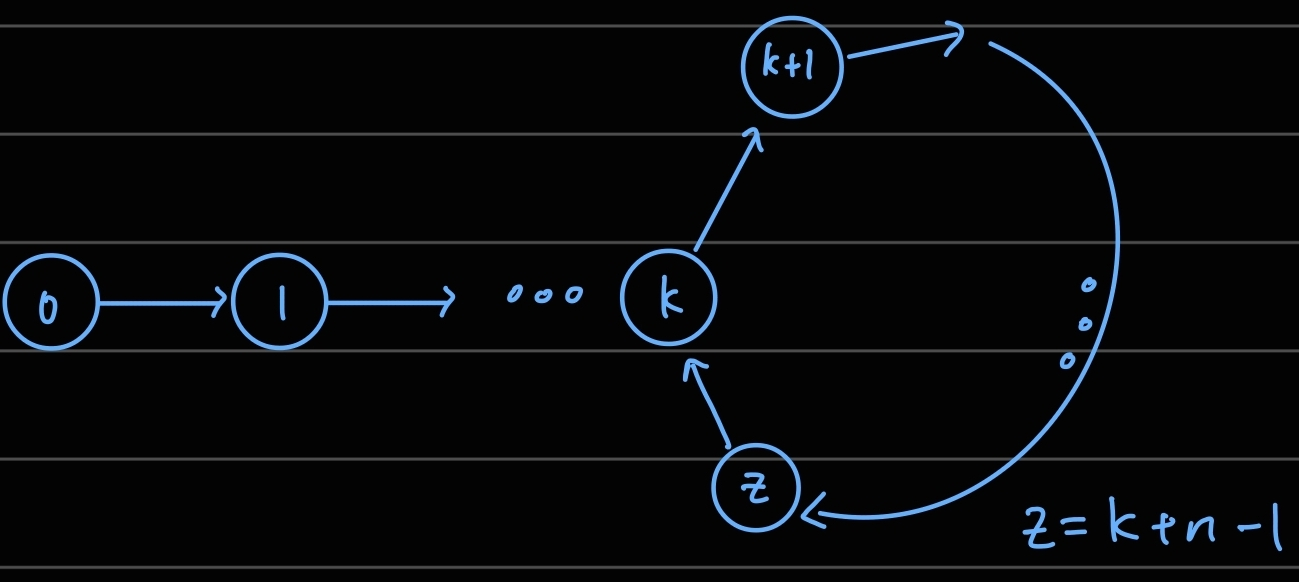
\includegraphics[width=8cm]{rsrc/floyd.jpg}
\end{center}
\item Let $p_s$ and $p_f$ represent the positions of the slow and fast pointers respectively.
\item Initially, $p_s = 0, p_f = 0.$
\item At $p_s = k$, $p_f = 2k$.
\item $\implies c = (2k-k) \% n = k \% n$ is the offset of the fast pointer when the slow pointer reaches the start of the cycle.
\item When, after m iterations, $p_s = k+m, p_f = 2(k+m)$ and $(p_s-k) == (p_f-k) \% n$.
\item $\implies (m + k) \% n = 0 \implies $ their current offsets in the cycle are (n-k)\% n.
\item $\implies $ If $p_a$ (new pointer) is $=0$, with k more iterations, the slow pointer's would be at $n-k + k = n$ (start of the cycle), as will $p_a$.
\end{itemize}
\section*{Misc. Notes}
\subsection*{Precision printing}
\begin{lstlisting}
cout.setf(ios_base::fixed,ios_base::floatfield);
cout.precision(<d>);//to print d digits after dp.
cout<<a;
//or
printf("%.<d>f",a);
\end{lstlisting}
\end{document}